%======================================================================
\NEWSEC
%======================================================================

\subsection{\ssInstallCharm}


\begin{frame}[fragile,label=ss-install-charm] 
\secframetitle{\ssInstallCharm}
\framesubtitle{Charm++ website: \urltext{http://charm.cs.illinois.edu}}
You will likely have to download and install Charm++ yourself
\begin{center}
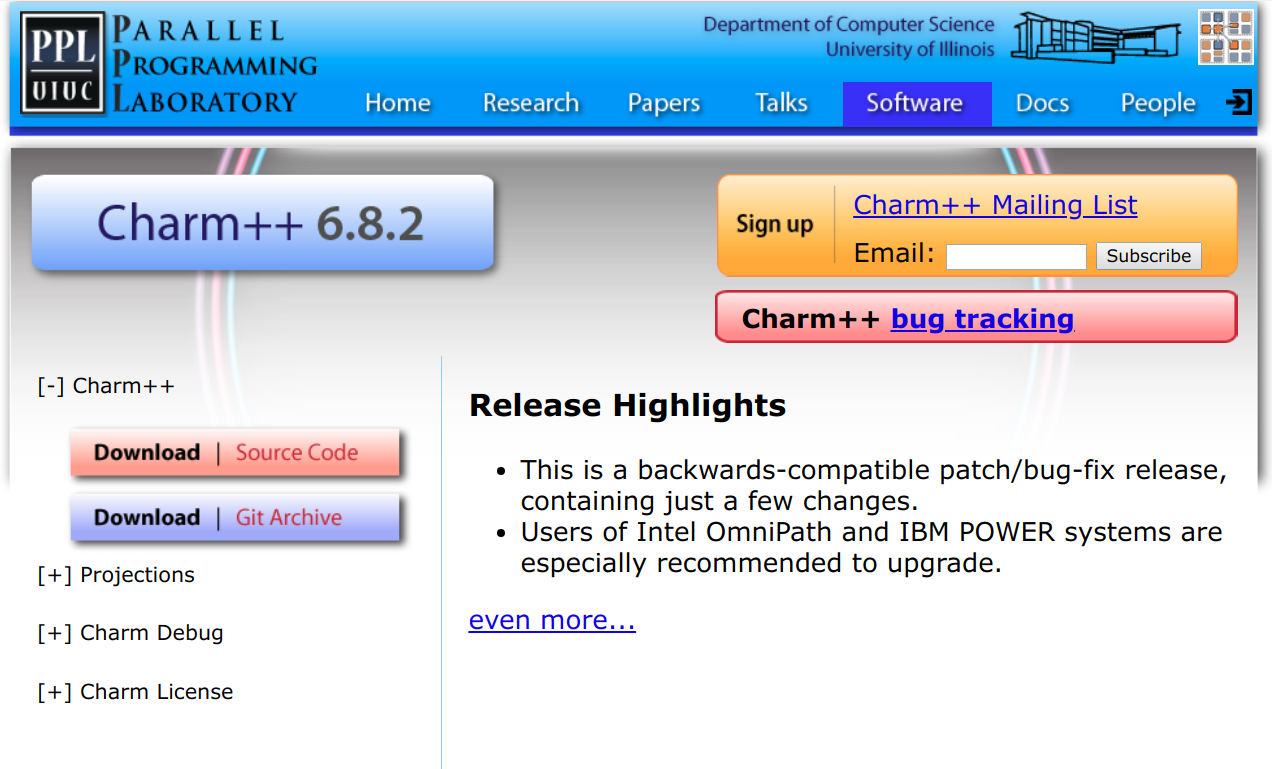
\includegraphics[width=4.00in]{charm-download.png}
\end{center}
\end{frame}


\setbeamercolor{block title}{bg=blue!30,fg=black}

%\usebackgroundtemplate
%{\includegraphics[width=5in]{monitor-2.png}}

\setbeamercolor{monitor-2.png}{bg=RGB{43,43,51}}

%----------------------------------------------------------------------

\begin{frame}[fragile] 
\secframetitle{\ssInstallCharm}
\color{black}
\footnotesize
%\begin{center}
%\begin{minipage}{3.3in}
%\begin{block}<+->{\textbf{Install \charm}}
\prompt             \redcode{ mkdir \url{~}/Charm}\cursor{1}  \\
\uncover<2->{\prompt\redcode{ cd \url{~}/Charm}\cursor{2}}  \\
\uncover<3->{\prompt\redcode{ wget http://charm.cs.illinois.edu/distrib/charm-6.8.2.tar.gz}\cursor{3}}  \\
\uncover<4->{\prompt\redcode{ tar zxf charm-6.8.2.tar.gz}\cursor{4}}  \\
\uncover<5->{\prompt\redcode{ ln -s charm-6.8.2 charm}\cursor{5}}  \\
\uncover<6->{\prompt\redcode{ cd charm}\cursor{6}}  \\
\uncover<7->{\bluecode{\# To build directly (recommended for Mac's)}} \\
\uncover<7->{\prompt\redcode{ ./build charm++ netlrts-darwin-x86\_64 gcc gfortran -j4 --with-production}\cursor{7}} \\
\uncover<8->{\bluecode{\# To build directly (recommended for Linux)}} \\
\uncover<8->{\prompt\redcode{ ./build charm++ netlrts-linux-x86\_64   -j4  --with-production}\cursor{8}} \\
\uncover<9->{\bluecode{\# To run the interactive build script:}} \\
\uncover<9->{\prompt\redcode{ ./smart-build.pl}\cursor{9}} \\
%\end{block}
%\end{minipage}
%\end{center}
\end{frame}


%----------------------------------------------------------------------

\begin{frame}[fragile] 
\secframetitle{\ssInstallCharm}
\framesubtitle{Compiling \charm\ with \code{./smart-build.pl}}
\color{black}
\footnotesize

\prompt\redcode{./smart-build.pl}\cursor{1}
\pause

\verb@============================================================@ \\
\ \\
\verb@Begin interactive charm configuration ...@\\
\verb@If you are a poweruser expecting a list of options, please use@ \\
\verb@   ./build --help@\\
\ \\
\verb@============================================================@ \\
\ \\
\verb@Are you building to run just on the local machine, and not across@ \\
\verb@multiple nodes? [y/N]@\cursor{2} \\
\pause
\verb@I found that you have an mpicc available in your path.@ \\
\verb@Do you want to build Charm++ on this MPI? [y/N]:@\cursor{3} \\
\end{frame}

%----------------------------------------------------------------------

\begin{frame}[fragile] 
\secframetitle{\ssInstallCharm}
\framesubtitle{Compiling \charm\ with \code{./smart-build.pl}}
\color{black}
\footnotesize

\verb@Do you have a special network interconnect? [y/N]:@\cursor{1}
\pause
\verb@y@ \\
\verb@	Choose an interconnect from below: [1-10]@ \\
\verb@		 1) MPI@ \\
\verb@		 2) Infiniband (ibverbs)@ \\
\verb@		 3) Cray XE, XK@ \\
\verb@		 4) Cray XC@ \\
\verb@		 5) Blue Gene/Q@ \\
\verb@		 6) Intel Omni-Path (ofi)@ \\
\verb@  @\cursor{2}
\end{frame}

%----------------------------------------------------------------------

\begin{frame}[fragile] 
\secframetitle{\ssInstallCharm}
\framesubtitle{Compiling \charm\ with \code{./smart-build.pl}}
\color{black}
\footnotesize

\verb@How do you want to handle SMP/Multicore: [1-3]@ \\
\verb@      1) single-threaded [default]@ \\
\verb@      2) SMP@ \\
\verb@      3) POSIX Shared Memory@ \\
\verb@  @\cursor{1}
\pause
\ \\
\verb@Do you want to specify a compiler? [y/N]@\cursor{2}\pause\verb@n@ \\
\ \\
\verb@Do you want to specify any Charm++ build options, such as fortran@ \\
\verb@   compilers? [y/N]@\cursor{3} \\

\end{frame}

%----------------------------------------------------------------------

\begin{frame}[fragile] 
\secframetitle{\ssInstallCharm}
\framesubtitle{Compiling \charm\ with \code{./smart-build.pl}}
\color{black}
\footnotesize

\verb@Choose a set of compiler flags [1-5]@ \\
\verb@	1) none@ \\
\verb@	2) debug mode                      -g -O0@ \\
\verb@	3) production build [default]      --with-production@ \\
\verb@	4) production build w/ projections --with-production --enable-tracing@ \\
\verb@	5) custom@ \\
\verb@  @\cursor{1}
\pause
\ \\ \ \\
\verb@What do you want to build?@ \\
\verb@          1) Charm++ [default] (choose this if you are building NAMD)@ \\
\verb@          2) Charm++ and AMPI@ \\
\verb@          3) Charm++, AMPI, ParFUM, FEM and other libraries@ \\
\verb@  @\cursor{2}
\end{frame}

%----------------------------------------------------------------------

\begin{frame}[fragile] 
\secframetitle{\ssInstallCharm}
\framesubtitle{Compiling \charm\ with \code{./smart-build.pl}}
\color{black}
\footnotesize
\ \\
\verb@Do you want to compile in parallel?@ \\
\verb@        1) No@ \\
\verb@        2) Build with -j2@ \\
\verb@        3) Build with -j4@ \\
\verb@        4) Build with -j8 @ \\
\verb@        5) Build with -j16 [default]@ \\
\verb@        6) Build with -j32@ \\
\verb@        7) Build with -j@ \\
\verb@  @\cursor{1}
\ \\
\pause
\verb@We have determined a suitable build line is:@ \\
\verb@	./build charm++ net-linux-x86_64  -j4  --with-production@ \\
\ \\
\verb@Do you want to start the build now? [Y/n]@\cursor{2} \pause\code{y}\\
\verb@Building with: ./build charm++ net-linux-x86_64  -j4 --with-production@

\end{frame}


%----------------------------------------------------------------------

% \begin{frame}[fragile] 
% \secframetitle{\ssInstallCharm}
% \framesubtitle{Running a \charm\ test problem}
% \color{black}
% \footnotesize
% 
% \prompt\redcode{ cd examples/charm++/hello/1darray}\cursor{1}\\\pause
% \prompt\redcode{ make test}\cursor{2}\\\pause
% 
% \color{blue}
% \verb@ ./charmrun +p4 hello 10@ \\
% \color{black}
% \verb@	Charmrun> started all node programs in 1.296 seconds. @ \\
% \verb@	Converse/Charm++ Commit ID:  @ \\
% \verb@	Trace: traceroot: /home/bordner/Charm/682/gnu/net/charm-6.8.2/examples/charm++/hello/1darray/hello @ \\
% \verb@	Charm++> scheduler running in netpoll mode. @ \\
% \verb@	CharmLB> Load balancer assumes all CPUs are same. @ \\
% \verb@	Charm++> Running on 1 unique compute nodes (8-way SMP). @ \\
% \verb@	Charm++> cpu topology info is gathered in 0.001 seconds. @ \\
% \verb@	Running Hello on 4 processors for 10 elements @ \\
% \verb@	Hello 0 created @ \\
% \verb@	Hello 1 created @ \\
% \verb@	Hello 2 created @ \\
% \verb@	Hi[17] from element 0 @ \\
% \verb@	Hi[18] from element 1 @ \\
% \verb@	Hi[19] from element 2 @ \\
% \verb@	Hello 6 created @ \ldots
% \end{frame}

\usebackgroundtemplate
{}

